\pdfminorversion = 4
\documentclass[shortpres,aspectratio=43]{beamer}
\usetheme{CambridgeUS}

\setbeamertemplate{footline}
{
  \leavevmode%
  \hbox{%
  \begin{beamercolorbox}[wd=.333333\paperwidth,ht=2.25ex,dp=1ex,left]{author in head/foot}%
  \hspace*{4ex}\usebeamerfont{author in head/foot}Ethan Lew%~~\beamer@ifempty{\insertshortinstitute}{}{(\insertshortinstitute)}
  \end{beamercolorbox}%
  \begin{beamercolorbox}[wd=.333333\paperwidth,ht=2.25ex,dp=1ex,center]{title in head/foot}%
    \usebeamerfont{title in head/foot} \insertshortdate{}
  \end{beamercolorbox}%
  \begin{beamercolorbox}[wd=.333333\paperwidth,ht=2.25ex,dp=1ex,right]{date in head/foot}%
    \usebeamerfont{date in head/foot}
    \insertframenumber{} / \inserttotalframenumber\hspace*{2ex}
  \end{beamercolorbox}}%
  \vskip0pt%
}\part{title}
\beamertemplatenavigationsymbolsempty

%color specification-----------------------------------------------------
\definecolor{TUMblue}{RGB}{27, 94, 170}%{rgb}{0.00, 0.40, 0.74}
\definecolor{TUMgray}{rgb}{0.85, 0.85, 0.86}
\definecolor{TUMpantone285C}{rgb}{0.00, 0.45, 0.81}
\definecolor{TUMpantone300C}{RGB}{27, 94, 170} %uncorrected TUMpantone300C
\definecolor{lightblue}{RGB}{213,227,241}%{rgb}{0.7529,0.8118,0.9333}
\definecolor{darkgreen}{RGB}{0, 200, 0}
\definecolor{verydarkgreen}{RGB}{0 120 0}
\definecolor{SBred}{RGB}{150 0 0}

\setbeamercolor{block title}{fg=white, bg=SBred}
\setbeamercolor{block body}{bg=lightblue}
\setbeamertemplate{blocks}[rounded][shadow=true]

%------------------------------------------------------------------------
\setbeamercolor{frametitle}{bg=SBred, fg=white}
\setbeamercolor{palette primary}{bg=SBred, fg=white}%{fg=TUMblue,bg=TUMgray}
\setbeamercolor{palette secondary}{use=palette primary,bg=SBred, fg=white}
\setbeamercolor{palette tertiary}{use=palette primary,fg=white, bg=SBred}
\setbeamercolor{palette quaternary}{use=palette primary,fg=white, bg=SBred}

\setbeamercolor{title}{bg=SBred,fg=white}
\setbeamercolor{item projected}{use=item,fg=black,bg = lightblue}
\setbeamercolor{block title}{fg=white, bg=SBred}
\setbeamercolor{block body}{bg=white}
\setbeamertemplate{blocks}[rounded][shadow=true]

%------------------------------------------------------------------------
\setbeamertemplate{bibliography item}{\insertbiblabel}
\setbeamercolor{bibliography item}{parent=palette primary}
\setbeamercolor{bibliography entry author}{fg=TUMblue}

%------------------------------------------------------------------------
\setbeamertemplate{enumerate items}[bullet]

%------------------------------------------------------------------------
\usepackage{subfigure}
\usepackage{textpos} % for figure (logo) on slides
\usepackage{psfrag} % for \psfrag in figures
\usepackage{algorithm,algpseudocode} % for algorithm environment
\usepackage{booktabs} % for rulers in tables
\usepackage{units} % for units to values
\usepackage{tikz}
\usetikzlibrary{calc,arrows,arrows.meta, automata,positioning,backgrounds}
\usetikzlibrary{overlay-beamer-styles,patterns}
\usetikzlibrary{chains, trees, fit, tikzmark}
\usetikzlibrary{shapes.geometric, shapes.arrows, decorations.pathreplacing}
\usepackage{makecell}
\usepackage{pgfplots}
\usepackage{graphicx}
\usepackage{colortbl}
\usepackage{array}
\usepackage{booktabs}
\usepackage{multirow}
\usepackage{bbding}
\usepackage[export]{adjustbox}
\usepackage{pifont}

% Packages
\usepackage{relsize}
\usepackage{cite}
\usepackage{graphicx}
\usepackage{pstool}
\usepackage{svg}
\usepackage{amsmath}
\usepackage{amssymb}
\usepackage{booktabs}
\usepackage{multirow}
\usepackage{fancyvrb} 
\usepackage{changepage}
\usepackage{siunitx}
\usepackage[skip=5pt]{caption}
\usepackage{arydshln}
\usepackage{comment}
\usepackage{setspace}
\usepackage{scalerel}
\usepackage{enumitem}

% for code
\usepackage{minted}
\newminted{python}{}
\newmintinline{python}{}
\newcommand{\py}[1]{\pythoninline{#1}}

\usepackage{tikz}
\usetikzlibrary{calc,arrows,arrows.meta, automata,positioning,backgrounds}
\usetikzlibrary{overlay-beamer-styles,patterns}
\usetikzlibrary{chains, trees, fit, tikzmark}
\usetikzlibrary{shapes.geometric, shapes.arrows, decorations.pathreplacing}
\usetikzlibrary{%
    ,arrows
    ,arrows.meta
    ,calc
    ,fit
    ,hobby
    ,positioning
}
\usetikzlibrary{shadows.blur}
\usetikzlibrary{shapes.symbols}

\newcommand{\cmark}{\ding{51}}%
\newcommand{\xmark}{\ding{55}}%

\setbeamerfont{caption}{size=\tiny}


% TikZ ---------------
\tikzset{
	preEdge/.style={black, <-, shorten <=1pt, >=stealth', semithick, rounded corners=2pt},
	postEdge/.style={black, ->, shorten >=1pt, >=stealth', semithick, rounded corners=2pt},
	axes/.style={black, ->, >=stealth'}
}
\definecolor{setedgeblue}{rgb}{0.00, 0.45, 0.81}
\definecolor{setfaceblue}{rgb}{0.7529,0.8118,0.9333}
\definecolor{setedgegreen}{rgb}{0.00,0.50,0.00}
\definecolor{setfacegreen}{rgb}{0.4510,0.9020,0.4510}
\definecolor{setedgegray}{rgb}{0.50,0.50,0.50}
\definecolor{setfacegray}{rgb}{0.85,0.85,0.85}
\definecolor{setedgered}{rgb}{0.6992,0.1367,0.1367}
\definecolor{setfacered}{rgb}{0.8906,0.2617,0.2070}
\pgfdeclarelayer{nodelayer}  
\pgfdeclarelayer{edgelayer}   
\pgfsetlayers{edgelayer,nodelayer, main}
\definecolor{left} {HTML}{001528}
% --------------------

% --------------------

\newcommand{\arstretch}[1]{\renewcommand{\arraystretch}{#1}}
\newcolumntype{C}[1]{>{\centering\arraybackslash}m{#1}}

%-----------------------------------------------------------------------
\newcommand{\at}{\fontfamily{ptm}\selectfont @}
\newcommand{\ra}[1]{\renewcommand{\arraystretch}{#1}} %to change the row spacing in tables

\newcommand\blfootnote[1]{%
  \begingroup
  \renewcommand\thefootnote{}\footnote{#1}%
  \addtocounter{footnote}{-1}%
  \endgroup
}

\setbeamertemplate{headline}[default]

%-----------------------------------------------------------------------
\title[AutoKoopman]{AutoKoopman: A Toolbox for Automated System Identification via Koopman Operator Linearization}

% \author[Lew et al.]{Stanley Bak$^1$, Sergiy Bogomolov$^2$, Brandon Hencey$^3$, \\ Niklas Kochdumper$^1$, \underline{Ethan Lew}$^4$, and Kostiantyn Potomkin$^2$}

\author[Lew et al.]{\underline{Ethan Lew}$^1$, Abdelrahman Hekal$^2$, Kostiantyn Potomkin$^2$, Niklas Kochdumper$^3$, Brandon Hencey$^4$, Stanley Bak$^3$, Sergiy Bogomolov$^2$}

\institute[Galois Inc.]{$^1$Galois Inc., $^2$Newcastle University, \\$^3$ Stony Brook University, $^4$Air Force Research Laboratory}

\date[ATVA 2023]{}

%---------------------------------------------------------------------
\begin{document}

%% TUM logo
%\addtobeamertemplate{frametitle}{}{
%\includegraphics[height=0.65cm]{./figures/logo.png} % for aspectratio=43
%\begin{textblock*}{\textwidth}(.95\textwidth,-0.9cm) % for aspectratio=169
%\includegraphics[height=0.8cm]{./figures/logo.png} % for aspectratio=169
%\end{textblock*}}

\begin{frame}[plain]
    \titlepage
\end{frame}

% Slide 2: Motivations
\begin{frame}
\frametitle{Motivations}

\begin{itemize}
    \item<1-> Koopman linearization methods identify nonlinear continuous dynamical systems using observed data, useful design and assurance tasks.
\end{itemize}
\begin{center}
	    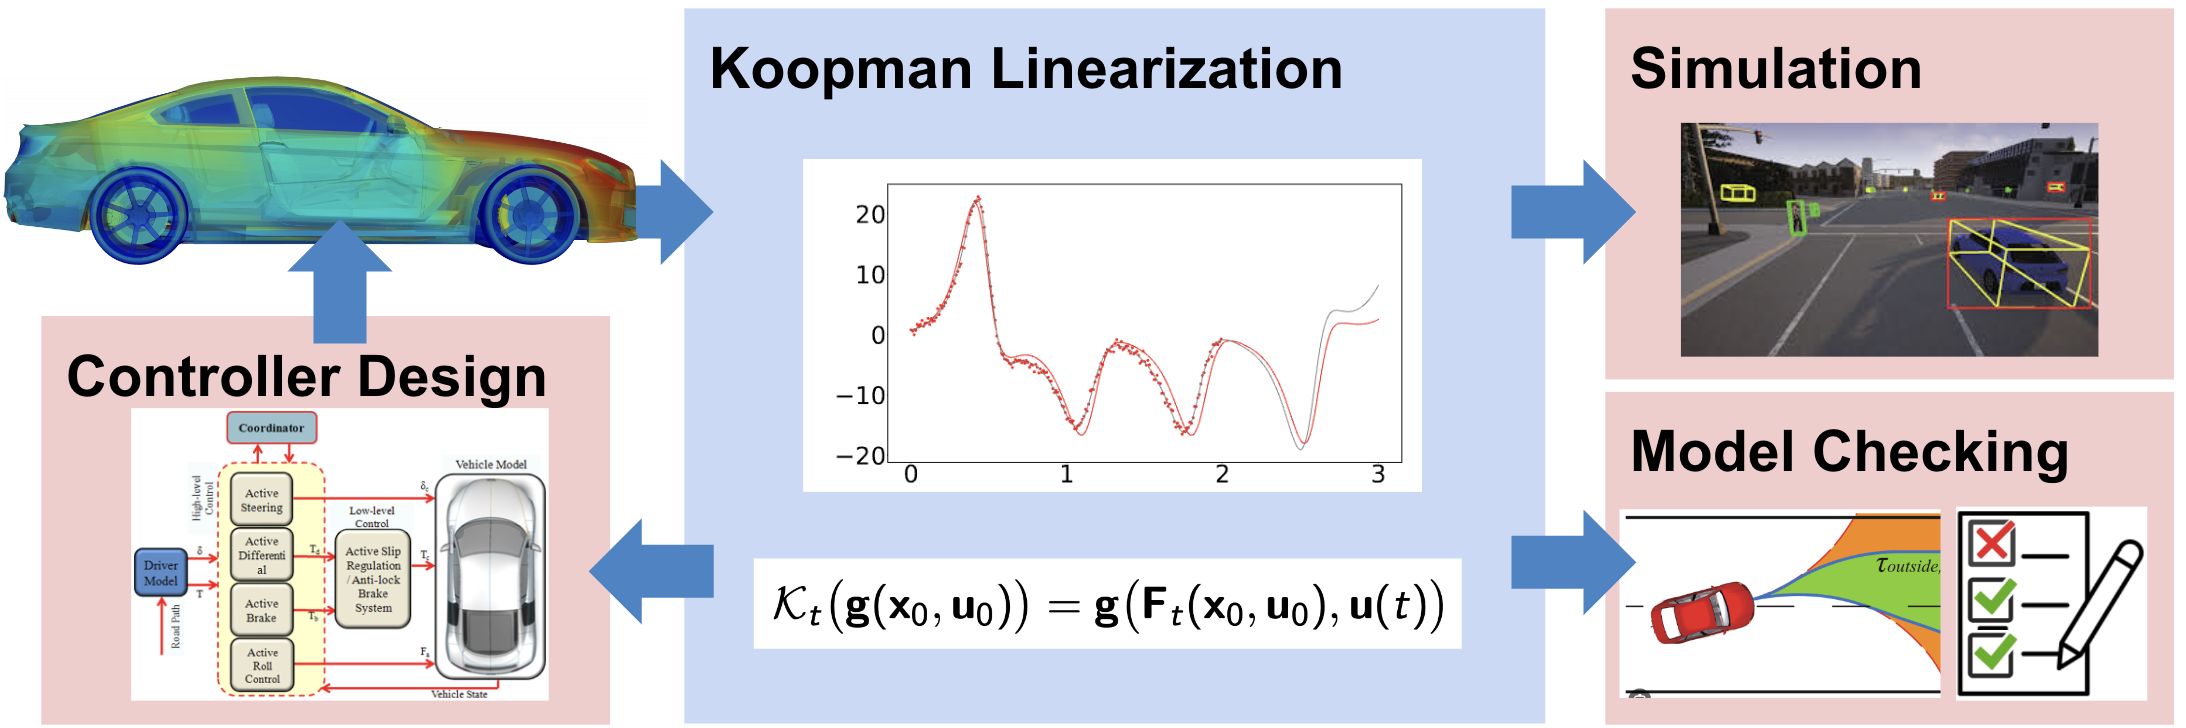
\includegraphics[width=0.95\linewidth]{./img/koopman.png}
    \end{center}
\begin{itemize}
    \item<2-> \textbf{Challenge:} System identification via Koopman linearization is complex, requiring careful selection of observables and hyperparameters.
    \item<3-> \textbf{Solution:} AutoKoopman automates this, optimizing all parameters to deliver an accurate Koopman linearized model.
\end{itemize}
\end{frame}

% Slide 3: System Identification Problem
\begin{frame}
\frametitle{System Identification Problem}
We aim to identify the dynamics of a continuous-time system 
\begin{equation*}
\dot{\mathbf x}(t) = \mathbf f(\mathbf x(t), \mathbf u(t))
\end{equation*}
with state $\mathbf x(t) \in \mathcal X \subseteq \mathbb R^n$ and input $\mathbf u(t) \in \mathcal U \subseteq \mathbb R^m$ from a set of $\numTraj{}$ trajectories \vspace{-5pt}
\begin{equation*}
\mathcal{T} = \big\{[(\mathbf x_i(t_0), \mathbf u_i(t_0)), \dots, \\ (\mathbf x_i(t_{\numMeas{}_i-1}), \mathbf u_i(t_{\numMeas{}_i-1}))] \big\}_{i=1}^{\numTraj{}}.
\end{equation*}
For now, we consider the uniform sampling case where $t_{i+1} = t_{i} + \Delta t$.
\rule{\textwidth}{1pt}
\begin{center}
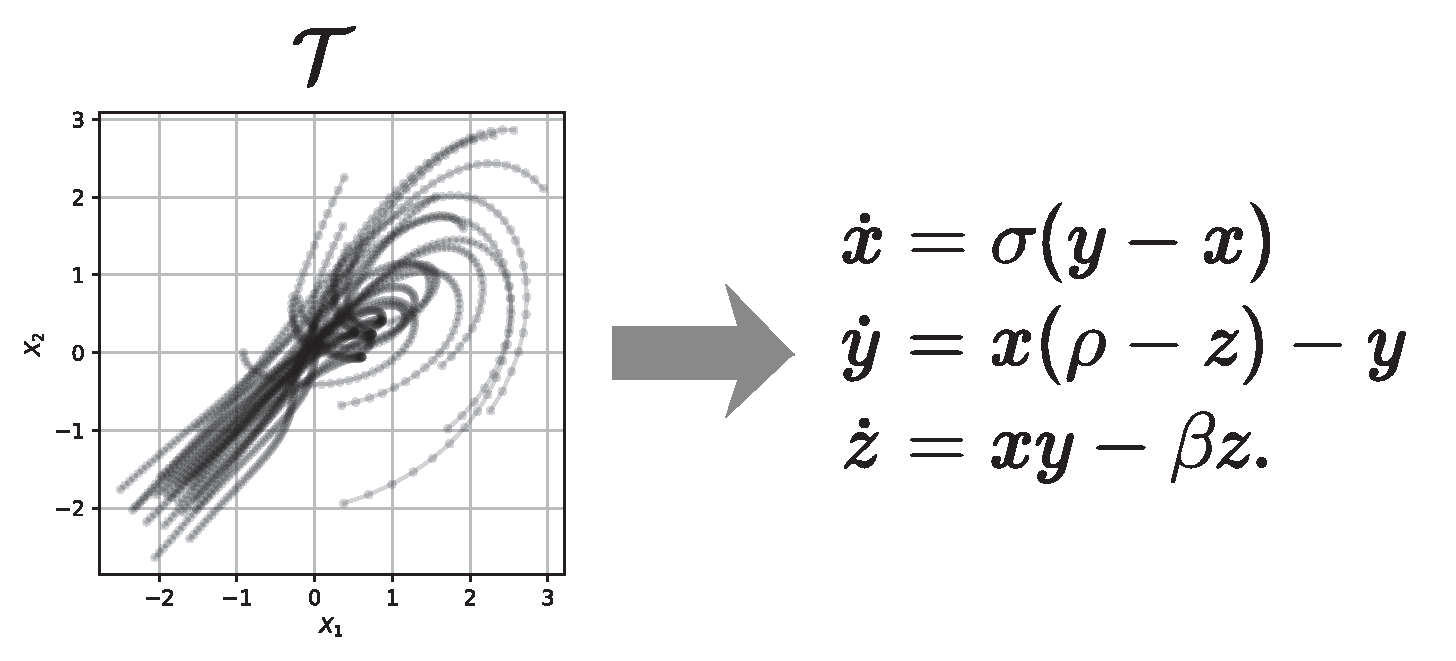
\includegraphics[width=0.7\linewidth]{./img/sysid.pdf}
\end{center}
\end{frame}

% Slide 4: The Koopman Operator
\begin{frame}
\frametitle{The Koopman Operator}
In 1931, B.O. Koopman introduced an alternative way to represent dynamic systems---a globally linear representation using a linear operator $\mathcal K_t$ on Koopman observables $\mathbf g(\mathbf x)$,
\[
\mathcal{K}_{t} \big(\mathbf{g} (\mathbf{x}_0, \mathbf{u}_0)\big) = \mathbf{g} \big(\mathbf{F}_{t}(\mathbf{x}_0,  \mathbf{u}_0 ), \mathbf{u}(t) \big)
\]

\begin{adjustbox}{max totalsize={.65\textwidth}{.65\textheight},center}
  \begin{tikzpicture}
    \begin{pgfonlayer}{nodelayer}
            \node [] (0) at (-4.25, 1.75) {}; 
            \node [] (1) at (-0.5, 1.25) {}; 
            \node [] (2) at (-6, -1.25) {}; 
            \node [] (3) at (-2.25, -1.75) {}; 
            \node [] (4) at (2.25, 1.75) {}; 
            \node [] (5) at (6, 1.25) {}; 
            \node [] (6) at (0.5, -1.25) {}; 
            \node [] (7) at (4.25, -1.75) {}; 
            \node [] (8) at (-0.75, 0) {}; 
            \node [] (9) at (0.75, 0) {}; 
            \node [] (12) at (0, 0) {$g$}; 
            \node [] (10) at (-1.55, 1.25) {$\mathcal M$}; 
            \node [] (11) at (5, 0.75) {$\mathcal H$};
            \node [] (13) at (-3, -0.1) {$F_t$};
            \node [] (14) at (3.2, -0.3) {$K_t$};
    \end{pgfonlayer}
    \begin{pgfonlayer}{edgelayer}
            \draw [shading=axis,fill=blue, opacity=0.3, left color=left, right color=left!10!white,shading angle=225] (0.center)
                     to [bend left] (1.center)
                     to [bend right=15] (3.center)
                     to [bend right] (2.center)
                     to [bend left, looseness=0.75] cycle;
            \draw [fill=blue, opacity=0.2] (4.center)
                     to (5.center)
                     to (7.center)
                     to (6.center)
                     to cycle;
            \draw [bend left, -stealth] (8.center) to (9.center);
    \end{pgfonlayer}
        \coordinate (g0) at (-5, 0);
        \coordinate (g1) at (-4.5, .5);
        \coordinate (g2) at (-4, -0.2);
        \coordinate (g3) at (-2.5, 1);
        \coordinate (g4) at (-2, 0);
      \draw [dashed, use Hobby shortcut]
      (g0) to [curve through = {(g1) .. (g2) .. (g3)}] (g4);
        \fill (g0) circle [radius=2pt] node [anchor=east] {$(x_0, u_0)$};
        \fill (g1) circle [radius=2pt] node [anchor=south] {$(x_1, u_1)$};
        \fill (g2) circle [radius=2pt] node [anchor=south] {$(x_2, u_2)$};
        \fill (g3) circle [radius=2pt] node [anchor=south] {$(x_3, u_3)$};
        \fill (g4) circle [radius=2pt] node [anchor=south] {$(x_4, u_4)$};

        \begin{scope}[xshift=6.5cm,yshift=-0.5cm]
        \coordinate (x0) at (-5, 0);
        \coordinate (x1) at (-4, .2);
        \coordinate (x2) at (-3.2, .7);
        \coordinate (x3) at (-2.5, 1);
        \coordinate (x4) at (-2, 0);
      \draw [dashed, use Hobby shortcut]
      (x0) to [curve through = {(x1) .. (x2) .. (x3)}] (x4);
        \fill (x0) circle [radius=2pt] node [anchor=south] {$y_0$};
        \fill (x1) circle [radius=2pt] node [anchor=south] {$y_1$};
        \fill (x2) circle [radius=2pt] node [anchor=south] {$y_2$};
        \fill (x3) circle [radius=2pt] node [anchor=south] {$y_3$};
        \fill (x4) circle [radius=2pt] node [anchor=south] {$y_4$};
        \end{scope}
\end{tikzpicture}
\end{adjustbox}

\pause
We aim to identify systems by learning $\mathbf g$ and $\mathcal K_{\Delta t}$. Essential to this task is the optimization problem
\begin{equation}
    \underset{\mathbf{g}, K_{\Delta t}}{\operatorname{argmin}} \sum_{\left(\mathbf{x}_k, \mathbf{u}_k\right) \in \mathcal{T}}\left\|\mathbf{g}\left(\mathbf{x}_{k+1}, \mathbf{u}_{k+1}\right)-K_{\Delta t} \mathbf{g}\left(\mathbf{x}_k, \mathbf{u}_k\right)\right\|_{\mathrm{MSE}}.
\end{equation}
\end{frame}

%Slide 8
\begin{frame}[fragile]
\frametitle{AutoKoopman Features}

AutoKoopman is high-level tool that automatically optimizes all hyper-parameters to obtain an accurate Koopman linearized models through a single function call
\rule{\textwidth}{1pt}
\begin{scriptsize}
\begin{minted}{python}
from autokoopman import auto_koopman

experiment_results = auto_koopman(
   training_data,    # list of trajectories
   obs_type="rff",   # random Fourier feature observables
   opt="bopt"        # auto-tuning via bayesian optimization
)      
\end{minted}
\end{scriptsize}
\rule{\textwidth}{1pt}

This accesses the toolboxes's major features
\begin{itemize}
	\item \textbf{System Identification}: eDMD, SINDy, Streaming, KIC
	\item \textbf{Observables}: Polynomial, Random Fourier Features, Neural Network
	\item \textbf{Hyperparameter Tuning}: Random, Grid Search, Bayesian Optimization
\end{itemize}

%\begin{itemize}
%    \item<1-> \textbf{SOTA Koopman Algorithms:} Access to various methods, including Deep Learning.
%    \item<2-> \textbf{Method Support:} Discrete-time, continuous-time system identification, and variations.
%    \item<3-> \textbf{Static Observables:} Different approaches for system observation.
%    \item<4-> \textbf{System Identification:} Techniques with input and control considerations.
%    \item<5-> \textbf{Online Identification:} Streaming system identification strategies.
%    \item<6-> \textbf{Hyperparameter Optimization:} Multiple strategies for efficient model tuning.
%\end{itemize}
\end{frame}

%Slide 5
\begin{frame}
\frametitle{F1Tenth Case Study: Problem Setup}
\begin{columns}
	\begin{column}{0.5\textwidth}
	\begin{itemize}
	    \item<1-> \textbf{F1Tenth Competition:} Open-source autonomous 1:10 scale car platform offering global competitions with innovative entries.
	    \item<3-> \textbf{Objective:} A Koopman linearized \textit{surrogate model} for control tasks and runtime assurance.
	    \item<4-> \textbf{Data Collection:} 21 Trajectories of the 4D vehicle state with 2D inputs collected for analysis.
	\end{itemize}
	\vspace{50pt}
	\end{column}
	\begin{column}{0.4\textwidth}
		\begin{figure}
		\centering
		  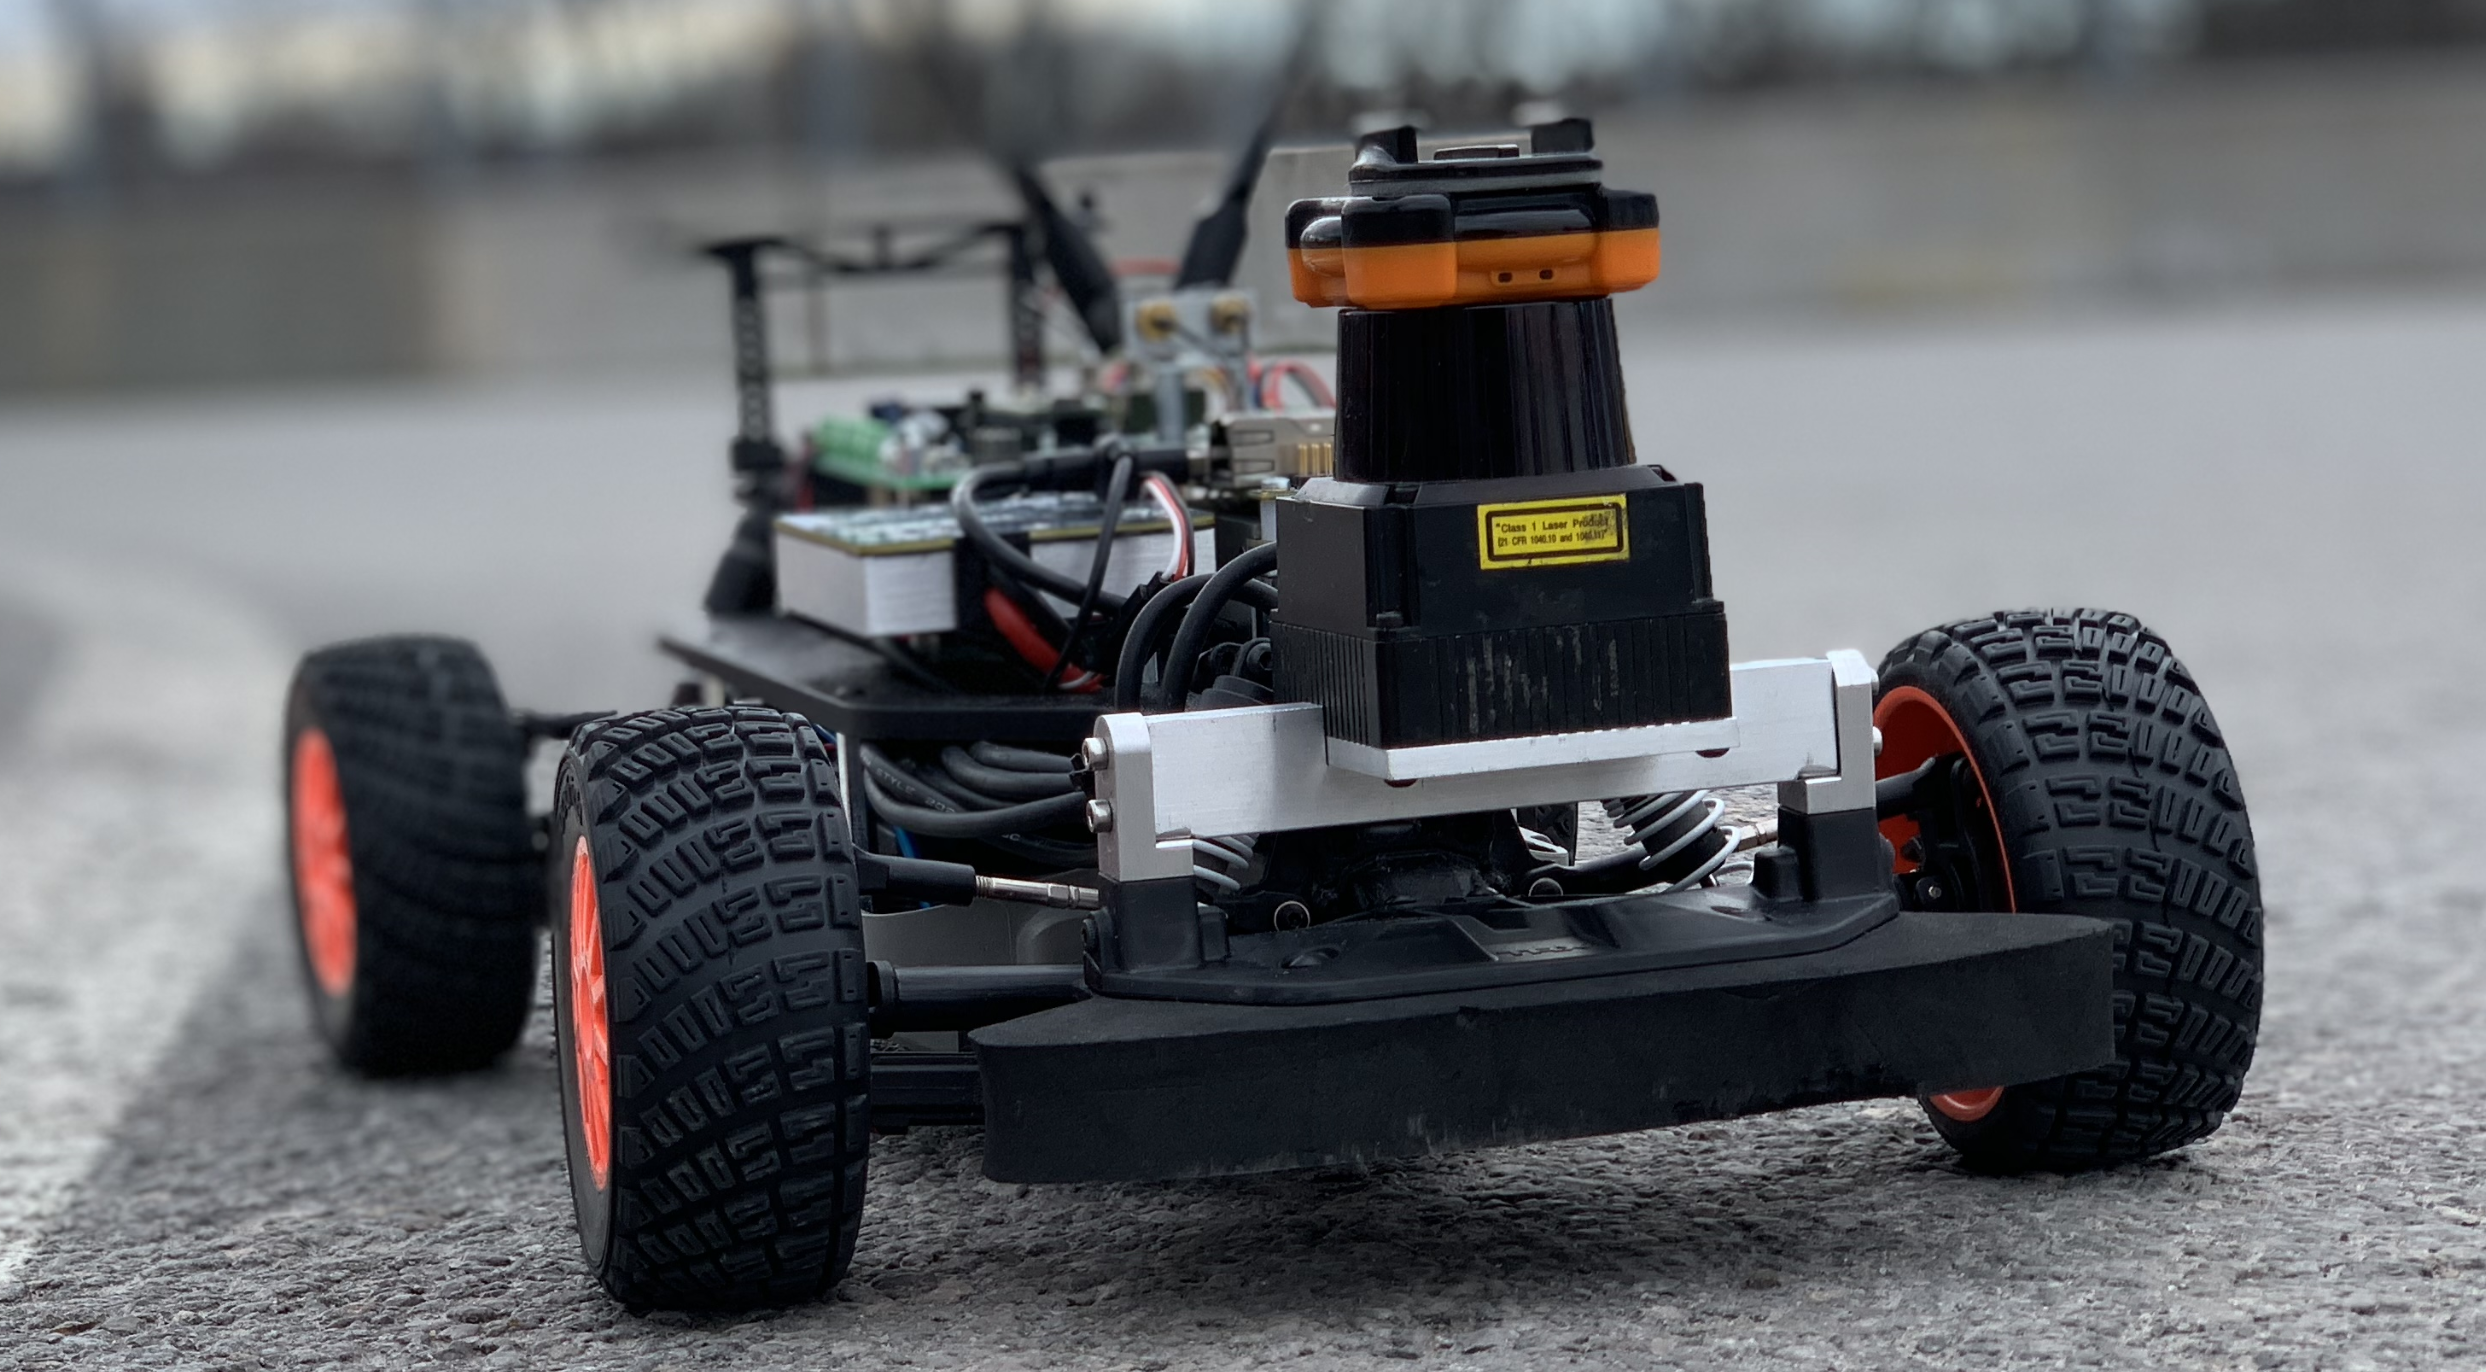
\includegraphics[width=0.9\textwidth]{./img/f1tenth.png}
		  \caption{The F1Tenth Platform}
		\end{figure}
		\begin{figure}
	\centering
	  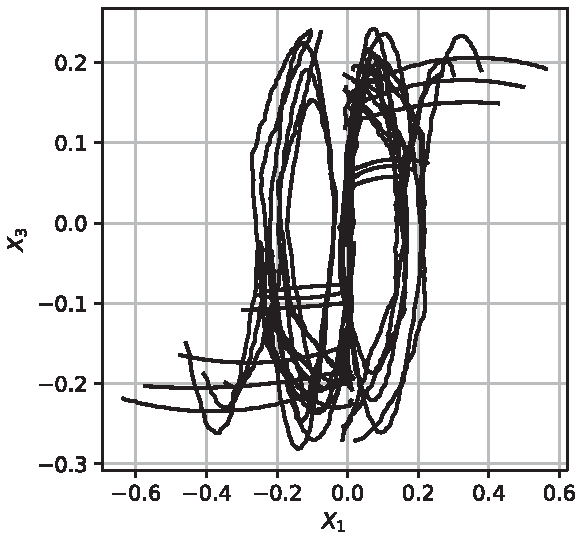
\includegraphics[width=0.8\textwidth]{./img/training.pdf} % replace 'path_to_image2' with the actual file path
	  \caption{Trajectories Data}
		\end{figure}
	\end{column}
\end{columns}
\end{frame}

%Slide 6
\begin{frame}
\frametitle{F1Tenth Case Study: Koopman Linearization and Tuning}
A convenience function allows us to experiment with many Koopman Linearization options, automatically tuning different hyperparameters involved. 
\rule{\textwidth}{1pt}
\vspace{-0.25cm}
\begin{columns}
	\begin{column}{0.32\linewidth}
		\small
		\textbf{Default Fit (RFFs)}
		\begin{itemize}
			\item $n$ observables: 42
			\item Score: 0.0432
		\end{itemize}
		\begin{center}
		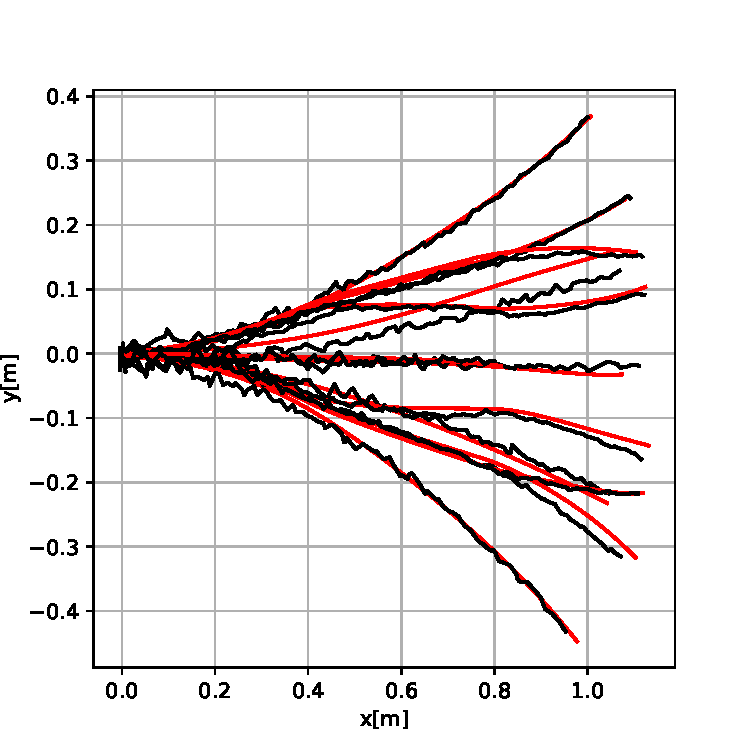
\includegraphics[width=0.8\linewidth]{./img/predictions.pdf}
		\end{center}
	\end{column}
	\begin{column}{0.32\linewidth}
		\small
		\textbf{Physical Priors (Handcrafted + RFFs)}
		\begin{itemize}
			\item $n$ observables: 42
			\item Score: 0.0371
		\end{itemize}
		\begin{center}
		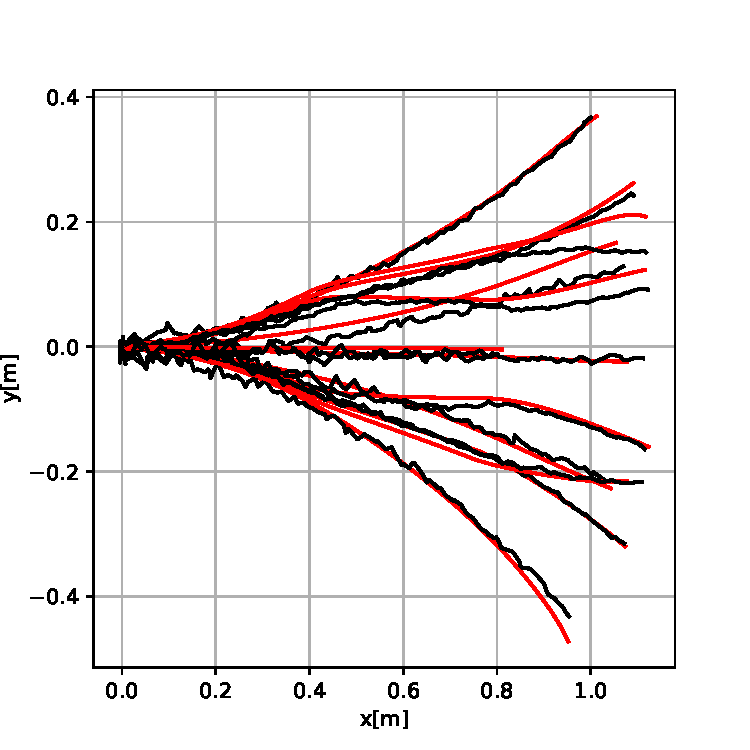
\includegraphics[width=0.8\linewidth]{./img/predictions_both.pdf}
		\end{center}
	\end{column}
	\begin{column}{0.32\linewidth}
		\small
		\textbf{Deep Learning (Autoencoder)}
		TODO
		\begin{itemize}
			\item $n$ observables: 42
			\item Score: 0.0432
		\end{itemize}
		\begin{center}
		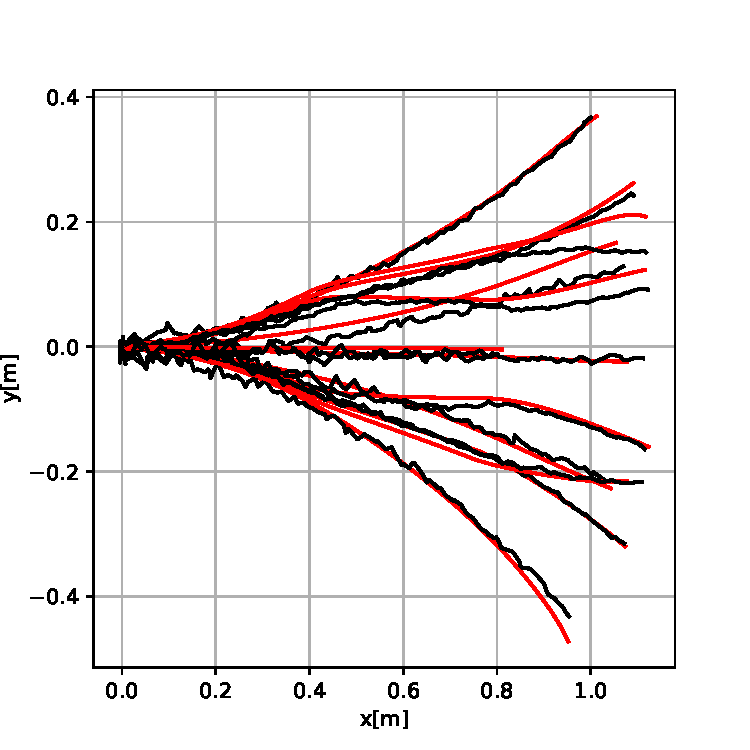
\includegraphics[width=0.8\linewidth]{./img/predictions_both.pdf}
		\end{center}
	\end{column}
\end{columns}
%\begin{rows}
%	\begin{row}{0.2\textheight}
%		A
%	\end{row}
%	\begin{row}{0.8\textheight}
%		B
%	\end{row}
%\end{rows}

% \begin{itemize}
%     \item<1-> \textbf{Observables Selection:} Initial phase crucial for model efficiency.
%     \item<2-> \textbf{Tuning Methodologies:} 
%     \begin{itemize}
%         \item Random Fourier Features.
%         \item Deep Learning techniques.
%         \item Integration of physical priors via Lie Derivatives.
%     \end{itemize}
% \end{itemize}
% % Placeholder for example python code
% \begin{figure}
%   \centering
%   \includegraphics[width=0.5\textwidth]{path_to_code_image} % replace 'path_to_code_image' with the actual file path
%   \caption{Example Python code}
% \end{figure}
% % Placeholder for accuracy plot
% \begin{figure}
%   \centering
%   \includegraphics[width=0.5\textwidth]{path_to_accuracy_plot} % replace 'path_to_accuracy_plot' with the actual file path
%   \caption{Accuracy plot}
% \end{figure}
\end{frame}

%Slide 7
\begin{frame}[fragile]
\frametitle{F1Tenth Case Study: Design and Analysis}
\begin{itemize}
    \item<1-> The Koopman Operator can be used for design and analysis tasks.
	    \vspace{12pt}
\begin{scriptsize}
    \begin{verbatim}
>> model.koopman_operator
array([[-2.25620904e+00,  2.62211614e+00,  3.09688097e+00, ...,
         1.76720882e-01,  9.64657948e-01,  1.07107764e-03],
       ...,
       [ 5.78220623e-01,  5.88793167e-02,  5.02129287e-01, ...,
         1.03782853e-01, -6.61264003e-01, -1.55678643e+00]])
    \end{verbatim}
    \end{scriptsize}
    %\item<2-> \textbf{Model Predictive Control (MPC):} Implemented using CasADi for enhanced control.
    %\item<3-> \textbf{Online Reachability:} Real-time analysis for runtime assurance.
\end{itemize}
\rule{\textwidth}{1pt}
\vspace{-0.25cm}
\begin{columns}
	\begin{column}{0.55\linewidth}
\textbf{Model Predictive Control (MPC)} 
\begin{figure}
	\centering
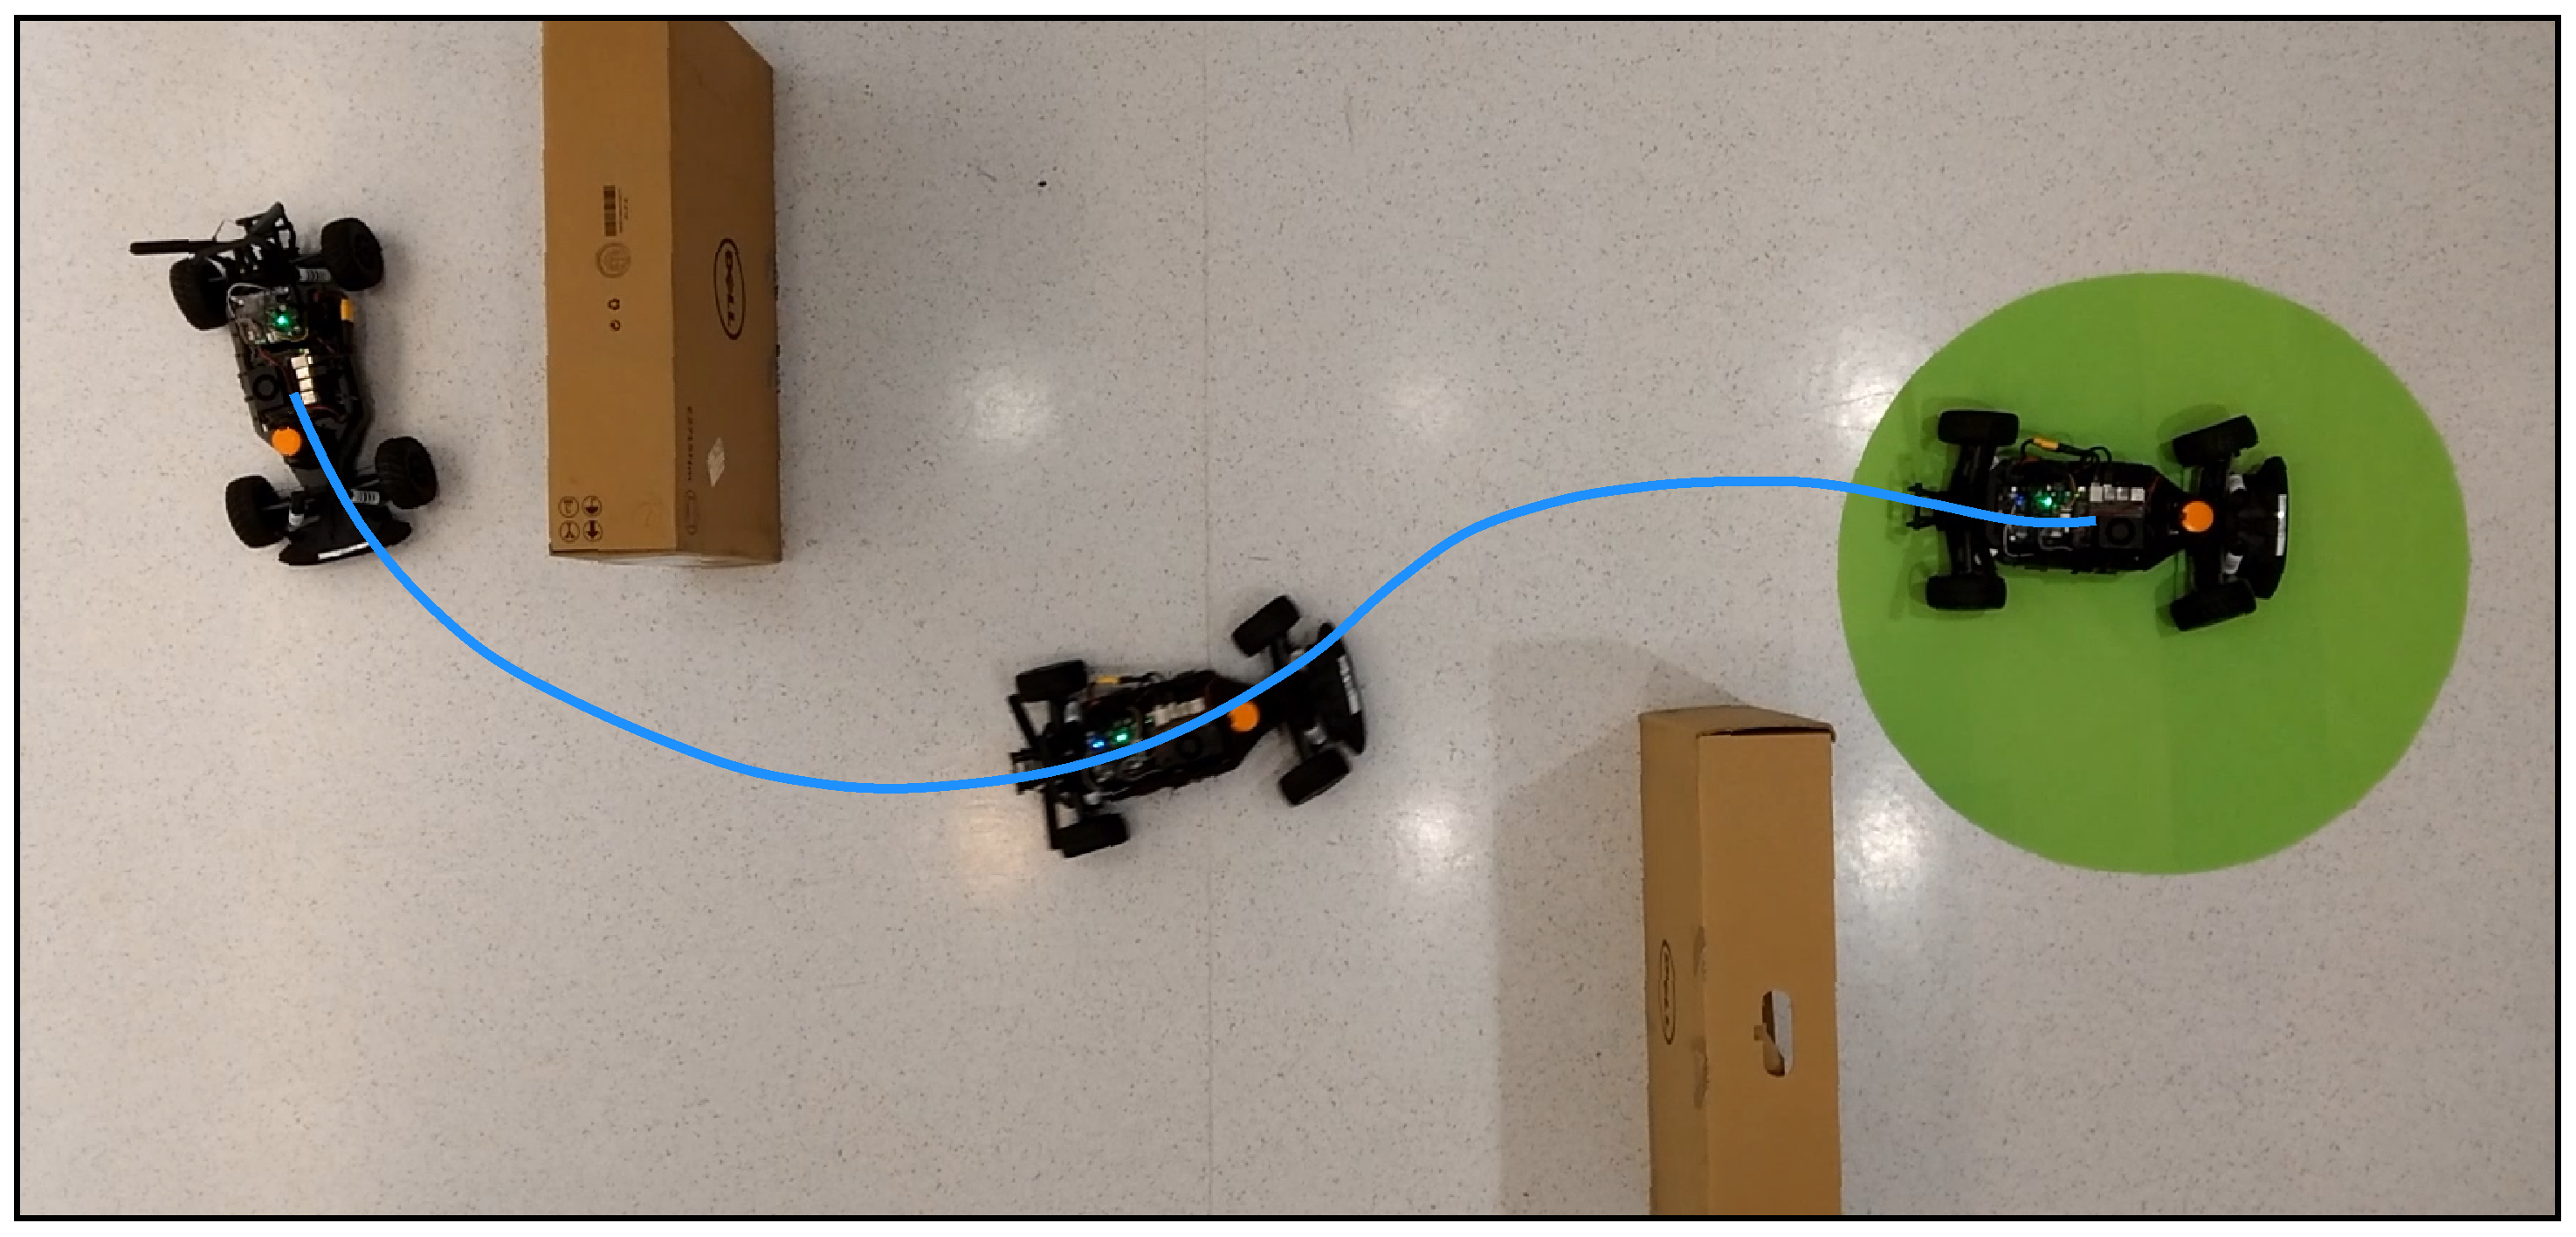
\includegraphics[width=0.8\linewidth]{./img/F1tenth.eps}
\caption{F1Tenth Koopman MPC}
\end{figure}
	\end{column}
	\begin{column}{0.45\linewidth}
\textbf{Online Reachability:} TODO
\end{column}
\end{columns}
\end{frame}

%Slide 9
\begin{frame}
\frametitle{Toolbox Architecture}
\begin{itemize}
    \item<1-> \textbf{Training Pipeline:} Architecture follows system identification training pipeline.
\end{itemize}
\begin{figure}
  \centering
  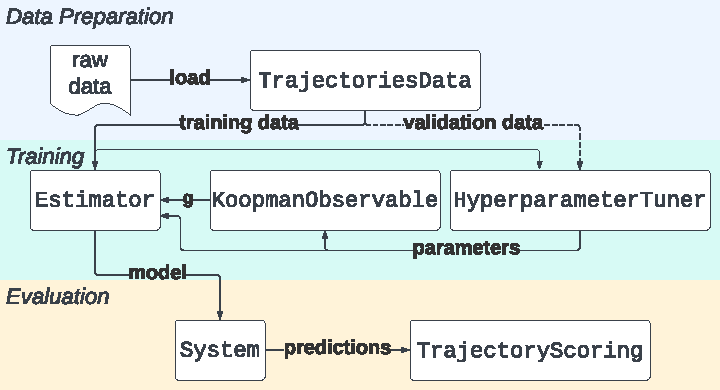
\includegraphics[width=0.7\textwidth]{./img/autokoopman_objects.pdf} % replace with actual file path
  \caption{System Architecture}
\end{figure}
\begin{itemize}
    \item<2-> \textbf{Extensibility:} Customize pipelines with unique observables, pre-processing, tuners, etc.
\end{itemize}
% Placeholder for architecture diagram
\end{frame}

%Slide 10
\begin{frame}
\frametitle{Benchmarks}
%\begin{itemize}
%    \item<1-> \textbf{Testing Parameters:} Evaluated on symbolic, black box, and real data benchmarks.
%    \item<2-> \textbf{Performance:} Effective across various types of observables.
%    \item<3-> \textbf{Improvements:} Enhanced performance over standard DMD.
%\end{itemize}
AutoKoopman has been evaluated on symbolic, black box, and real data benchmarks.
\begin{table*}%[!tb]
\begin{center}
\renewcommand{\arraystretch}{1.3}
\caption{Comparison of the constructed Koopman linearized models.}
\label{tab:benchmarks}
%\vspace{-0.25cm}
%\resizebox{\textwidth}{!}{%
\tiny
\begin{tabular}{c l c c c c c c c c c c c c c}
\toprule
& \textbf{System} & & \multicolumn{2}{c}{\textbf{Baseline}} & & \multicolumn{2}{c}{\textbf{Polynomial}} & & \multicolumn{2}{c}{\textbf{Fourier}} & & \multicolumn{2}{c}{\textbf{Neural Net.}} \\ \cmidrule{4-5} \cmidrule{7-8} \cmidrule{10-11} \cmidrule{13-14}
 & & \hspace{3pt} dims \hspace{3pt} & error & time & ~ & error & time & ~ & \hspace{3pt} error \hspace{3pt} & time & ~ & \hspace{3pt} error \hspace{3pt} & time \\ \midrule
 \multirow{7}{*}{\rotatebox[origin=c]{90}{\textbf{symbolic}}} & ~Pendulum 
 & 2 & 21.4\% & 0.30 & ~ & 1.37\% & 14.8 & ~ & \textbf{1.62\%} & 16.4 & ~ & 43.2\% & 114\\
 & ~FitzHugh-Nagumo
 & 2 & 49.6\% & 0.18 & ~ & 35.6\% & 6.23 & ~ & \textbf{0.55\%} & 15.2 & ~ & 67.8\% & 147	\\
 & ~Robertson 
 & 2 & \textbf{6.43\%} & 0.19 & ~ & \textbf{6.43\%} & 2.79 & ~ & 26.0\% & 15.0 & ~ & 19.23\% & 173	\\
  & ~Production-Destruction  
  & 2 & 26.5\% & 0.19 & ~ & 26.5\% & 2.77 & ~ & \textbf{2.07\%} & 15.31 & ~ & 59.3\% & 323\\
  & ~Spring Pendulum 
  & 4 & 89.7\% & 0.19 & ~ & 89.7\% & 3.73 & ~ & \textbf{0.03\%} & 15.6 & ~ & 8.6\% & 98.2 \\
 & ~Laub-Loomis 
 & 7 & 5.47\% & 0.26 & ~ & 0.21\% & 9.82 & ~ & \textbf{0.04\%} & 16.0 & ~ & 22.25\% & 92.4 \\
 & ~Biological Model
 & 9 & 0.06\% & 0.35 & ~ & 0.06\% & 4.81 & ~ & \textbf{0.01\%} & 15.7 & ~ & 22.3\% & 178 \\
 & ~Trans. Regulator Network
 & 48 & 27.5\% & 0.53 & ~ & 27.5\% & 4.57 & ~ & 4.60\% & 18.4 & ~ & \textbf{3.11\%} & 165\\ \vspace{-10pt} \\ 
\hdashline \vspace{-10pt} \\
 \multirow{3}{*}{\rotatebox[origin=c]{90}{\textbf{sim}}} & ~Engine Control 
 & 2 & 13.5\% & 3.25 & ~ & 13.5\% & 40.2 & ~ & \textbf{2.54\%} & 119 & ~ & 22.9\% & 429 \\\
 & ~Longitudinal Control
 & 7 & 3.24\% & 0.32 & ~ & 3.24\% & 2.09 & ~ & \textbf{0.00\%} & 35.9 & ~ & 3.13\% & 164 \\
 & ~Collision Avoidance 
 & 16 & 2.61\% & 13.1 & ~ & 2.61\% & 236 & ~ & \textbf{2.39\%} & 600 & ~ & 95.1\% & 849\\ \vspace{-10pt} \\ 
\hdashline \vspace{-10pt} \\
 \multirow{3}{*}{\rotatebox[origin=c]{90}{\textbf{real}}} & ~Electric Circuit
 & 3 & \textbf{14.4\%} & 25.1 & ~ & \textbf{14.4\%} & 2217 & ~ & \textbf{14.4\%} & 1609 & ~ & 14.9\% & 1240 \\
 & ~F1tenth Racecar
 & 4 & 64.1\% & 1.88 & ~ & 64.1\% & 53.9 & ~ & 60.1\% & 41.7 & ~ & \textbf{50.7\%} & 177  \\
 & ~Robot Arm 
 & 12 & 66.4\% & 11.1 & ~ & 66.4\% & 163 & ~ & 33.0\% & 517 & ~ & \textbf{23.9\%} & 360 \\
%
\bottomrule
\end{tabular}
%} %end of resizebox
\end{center}
\vspace{-22pt}
\end{table*}
\end{frame}

%Slide 11
\begin{frame}
\frametitle{Conclusion and Future Work}
\begin{itemize}
    \item \textbf{AutoKoopman Tool:} 
    \begin{itemize}
        \item Automated Koopman Linearized System.
        \item Extensibility and ease of use.
    \end{itemize}
    \item \textbf{Availability:} Hosted on platforms like GitHub and PyPI.
    \item \textbf{Future Work:} Potential integration with verification and control tools.
\end{itemize}
\end{frame}

\end{document}
